\documentclass[]{article}
\usepackage{lmodern}
\usepackage{amssymb,amsmath}
\usepackage{ifxetex,ifluatex}
\usepackage{fixltx2e} % provides \textsubscript
\ifnum 0\ifxetex 1\fi\ifluatex 1\fi=0 % if pdftex
  \usepackage[T1]{fontenc}
  \usepackage[utf8]{inputenc}
\else % if luatex or xelatex
  \ifxetex
    \usepackage{mathspec}
    \usepackage{xltxtra,xunicode}
  \else
    \usepackage{fontspec}
  \fi
  \defaultfontfeatures{Mapping=tex-text,Scale=MatchLowercase}
  \newcommand{\euro}{€}
\fi
% use upquote if available, for straight quotes in verbatim environments
\IfFileExists{upquote.sty}{\usepackage{upquote}}{}
% use microtype if available
\IfFileExists{microtype.sty}{%
\usepackage{microtype}
\UseMicrotypeSet[protrusion]{basicmath} % disable protrusion for tt fonts
}{}
\usepackage[margin=1in,a4paper]{geometry}
\usepackage{graphicx}
\makeatletter
\def\maxwidth{\ifdim\Gin@nat@width>\linewidth\linewidth\else\Gin@nat@width\fi}
\def\maxheight{\ifdim\Gin@nat@height>\textheight\textheight\else\Gin@nat@height\fi}
\makeatother
% Scale images if necessary, so that they will not overflow the page
% margins by default, and it is still possible to overwrite the defaults
% using explicit options in \includegraphics[width, height, ...]{}
\setkeys{Gin}{width=\maxwidth,height=\maxheight,keepaspectratio}
\ifxetex
  \usepackage[setpagesize=false, % page size defined by xetex
              unicode=false, % unicode breaks when used with xetex
              xetex]{hyperref}
\else
  \usepackage[unicode=true]{hyperref}
\fi
\hypersetup{breaklinks=true,
            bookmarks=true,
            pdfauthor={},
            pdftitle={},
            colorlinks=true,
            citecolor=blue,
            urlcolor=blue,
            linkcolor=magenta,
            pdfborder={0 0 0}}
\urlstyle{same}  % don't use monospace font for urls
\setlength{\parindent}{0pt}
\setlength{\parskip}{6pt plus 2pt minus 1pt}
\setlength{\emergencystretch}{3em}  % prevent overfull lines
\setcounter{secnumdepth}{0}

\usepackage{color}
\date{}

\begin{document}

\section{Response to reviewers}\label{response-to-reviewers}

\section{Reviewer 1}\label{reviewer-1}

\textbf{1. Reviewer's Comment:}

Introduction 1. Second paragraph, second sentence: The fact that the
Nymphalids are the ``largest family'' of butterflies conveys an
exaggerated importance of their diversity based on idiosyncrasy of
Linnean taxonomy (the sister group to Nymphalidae, the clade that
includes riodinids and lycaenids, has over 6500 species). Consider
revising the sentence, omitting superlatives (``biggest'', ``largest'',
``most'', etc.).

\textbf{1. Response:}

\begin{quote}
\color{blue}
We have rewritten the sentence to: ``Nymphalidae contains around 6000
species {[}6{]}, and several members are considered model organisms in
evolutionary biology {[}7--9{]}.''
\end{quote}

\textbf{2. Reviewer's Comment:}

The authors should mention that the ideal approach would accommodate
uncertainty by sampling from a distribution of trees which reflected the
variation in confidence in various parts of the tree (such as a Bayesian
posterior distribution or a bootstrap sample). See Holder,M. and
Lewis,P.O. (2003) Phylogeny estimation: traditional and Bayesian
approaches. Nat. Rev.~Genet., 4, 275--284

\textbf{2. Response:}

\begin{quote}
\color{blue}
We have specified that the sample of trees was taken from the Bayesian
run in Wahlberg et al., 2009.
\end{quote}

\textbf{3. Reviewer's Comment:}

Middle of paragraph (and throughout the manuscript): revise the tree
sampling to ``\ldots{}therefore randomly sampled 1000 trees from the
posterior distribution''; in the remainder of the manuscript, refer to
these as the ``1000 sampled trees'', not ``1000 random trees'', which
can take on a very different meaning.

\textbf{3. Response:}

\begin{quote}
\color{blue}
We have corrected some sentences in the manuscript to specify that we
are referring to the same set of 1000 trees.
\end{quote}

\textbf{4. Reviewer's Comment:}

Define what `MuSSE' refers to (Multiple State Speciation and
Extinction?).

\textbf{4. Response:}

\begin{quote}
\color{blue}
We have included the definition of MuSSE in the manuscript.
\end{quote}

\textbf{5. Reviewer's Comment:}

A reference for the statement ``most of Nymphalidae butterflies are
restricted to use one plant family as hostplant'' is warranted.

\textbf{5. Response:}

\begin{quote}
\color{blue}
We have included the numbers of single-family feeders based on
calculations of our own data on hostplant use across Nymphalidae genera.
The text has been modified accordingly:
\end{quote}

\begin{quote}
\color{blue}
``Because most of Nymphalidae butterflies are restricted to use one
plant family as hostplant (232 genera use only one plant family versus
176 that use more than one; based on our data in supp. mat. 15), the
\ldots{}''
\end{quote}

\textbf{6. Reviewer's Comment:}

At the end of this paragraph, the authors indicated they tested the
effect of character coding on their analyses. A more explicit
description of the test would be useful, along with predictions of how
results would be effected (i.e.~how would a large effect vs.~no effect
of coding Hypanartia and Vanessa as Solanaceae feeders manifest in the
results?).

\textbf{6. Response:}

\begin{quote}
\color{blue}
We included the following sentence to clarify the issue:\\\textbf{``We
expected that coding these two genera as either absence or presence
would not have a significant effect on our results.''}
\end{quote}

\textbf{7, 8, 9, 10. Reviewer's Comment:}

\begin{enumerate}
\def\labelenumi{\arabic{enumi}.}
\setcounter{enumi}{6}
\itemsep1pt\parskip0pt\parsep0pt
\item
  First paragraph, second sentence: change the tense of ``run'' to
  ``ran''.
\item
  Second paragraph, third sentence: replace ``Thus'' with
  ``Furthermore''.
\item
  There appears to be an orphaned right-parenthesis at the end of the
  second paragraph.
\item
  Third paragraph, last sentence: The node number is not really
  relevant, so beginning of the sentence could be revised to ``For
  example, the Charaxes + Polyura clade was found in only 256
  trees\ldots{}''
\end{enumerate}

\textbf{7, 8, 9, 10. Response:}

\begin{quote}
\color{blue}
We made the suggested corrections.
\end{quote}

\textbf{11. Reviewer's Comment:}

Fourth paragraph: The point of the paragraph is not clear. What rates
are being compared? MEDUSA vs.~MultiMEDUSA? Consider revising to make
the point clearer or omit the sentence.

\textbf{11. Response:}

\begin{quote}
\color{blue}
We have rewritten the sentence and now is more clear:\\\textbf{``For the
diversification shifts found in both the MCC tree and most of the
samples of 1000 trees (frequency more than 90\%; Table 2), the
MultiMEDUSA approach recovered different rates of diversification than
those found using when the MCC tree alone.''}.
\end{quote}

\textbf{12. Reviewer's Comment:}

Fifth paragraph, first sentence (and potentially elsewhere): Consider
using a consistent means of presenting probability values. In this
sentence, the authors refer to ``90\% of probability in the trees'', but
in the preceding paragraph, the authors present probabilities as a
decimal (``probability of being recovered higher than 0.90''). Granted,
these two probabilities refer to different events, but perhaps it would
be best to refer to them in a consistent manner, such as ``0.90
posterior probability''.

\textbf{12. Response:}

\begin{quote}
\color{blue}
We have corrected this and normalized the probability values to decimals
in the manuscript.
\end{quote}

\textbf{13. Reviewer's Comment:} The third sentence (length of analysis
and burnin details) should be moved to the methods section.

\textbf{13. Response:}

\begin{quote}
\color{blue}
We made the suggested corrections.
\end{quote}

\textbf{14. Reviewer's Comment:}

Mid-way through paragraph, discussion of likelihood ratio test: The
source of this P-value needs to be described (chi-squared approximation
with 1 degree of freedom?), here or in the methods section (see p.~617
in Pagel 1999 Syst. Biol. 48:612-622).

\textbf{14. Response:}

\begin{quote}
\color{blue}
We have include the statistics suggested by the reviewer:
``\textbf{\(\chi^2 = 12.3; 1 df; p < 0.001\)}''.
\end{quote}

\textbf{15. Reviewer's Comment:}

The closing three sentences (about BiSSE performance) should be moved to
the methods section.

\textbf{15. Response:}

\begin{quote}
\color{blue}
We made the suggested corrections.
\end{quote}

\textbf{16. Reviewer's Comment:}

First paragraph: The authors' assessment of analyzing diversification
shifts using a single tree, without accommodating our level of certainty
in relationships, is justified; however, MEDUSA itself, that is, the
approach using stepwise AIC to identify shifts in diversification rate,
should not be the target of criticism. After all, MultiMEDUSA is doing
the same thing, but on a sample of trees. Revise this paragraph with a
more appropriate target for the criticism (i.e.~analyses performed on
single trees).

\textbf{16. Response:}

\begin{quote}
\color{blue}
We have reworded the paragraph to avoid blaming the method:
\end{quote}

\begin{quote}
\color{blue}
``The MEDUSA method has been used to infer changes in net
diversification rates in a phylogenetic tree. Since its publication
{[}16{]} the results of using MEDUSA on a single tree, the maximum clade
credibility tree, have been used for generation of hypotheses and
discussion {[}10,42,43{]}. However, different diversification shifts and
different rates of diversification are found for certain lineages when
phylogenetic uncertainty was taken into account by using MEDUSA on a
random sample of trees from the posterior distribution of a Bayesian
run. We found that some diversification splits, estimated on the
Nymphalidae maximum clade credibility tree, were found with very low
probability in the random sample of 1000 trees from the posterior
distribution (Fig. 3, Table 2). We also found that, even though the
analyses estimated the same diversification splits on two or more trees,
the estimated net diversification rates could vary widely (Fig. 2).''
\end{quote}

\textbf{17. Reviewer's Comment:}

Seventh paragraph, second to last sentence: Two ages for Ithomiini are
given -- are they the origin and diversification ages? If so, revise the
sentence to include this information (rather than requiring readers to
refer to the preceding sentence): ``Reference 10 gives the ages of
origin and diversification for Ithomiini at 45 (39-53) and 37 (32-43)
MYA, respectively''.

\textbf{17. Response:}

\begin{quote}
\color{blue}
We have followed the reviewer's suggestion.
\end{quote}

\textbf{18. Reviewer's Comment:}

Eighth paragraph: This paragraph discussing biogeography does not fit
and could be omitted without detriment to the manuscript.

\textbf{18. Response:}

\begin{quote}
\color{blue}
We have followed the reviewer's suggestion and removed this paragraph.
\end{quote}

\textbf{19. Reviewer's Comment:}

First paragraph, first sentence: replace ``gave'' with ``showed''.

\textbf{19. Response:}

\begin{quote}
\color{blue}
We corrected the text following the reviewer's suggestion.
\end{quote}

\textbf{20. Reviewer's Comment:}

This section is predominantly speculative. Consider a more rigorous
discussion (if appropriate) or omit.

\textbf{20. Response:}

\begin{quote}
\color{blue}
We have followed the reviewer's suggestion and removed this paragraph.
\end{quote}

\textbf{21. Reviewer's Comment:}

First paragraph, second sentence: revise ``13\% of probabilities of the
trees from the posterior distribution'' to ``13\% of the trees from the
posterior distribution''.

\textbf{21. Response:}

\begin{quote}
\color{blue}
We corrected the text following the reviewer's suggestion.
\end{quote}

\textbf{22. Reviewer's Comment:}

Second paragraph: this paragraph is, for the most part, unnecessary. The
last sentence of the paragraph should be revised and appended to the end
of the preceding (first) paragraph: ``\ldots{}not picked up by MEDUSA.
This would be expected if the diversification of Satyrinae occurred in a
stepwise manner, with pulses or bursts of diversification for certain
lineages but unlikely for the tribe Satyrini as a whole''.

\textbf{22. Response:}

\begin{quote}
\color{blue}
We corrected the text following the reviewer's suggestion.
\end{quote}

\textbf{23. Reviewer's Comment:}

Final two paragraphs: There needs to be a section break, to indicate a
change in the discussion topic. ``Conclusions'' would be appropriate to
indicate to readers that these paragraphs represent a summary of the
major points of the work. The final paragraph is a good summary of the
work, and it would be a disservice to have readers miss it because it
appears under the `Satyrini' section.

\textbf{23. Response:}

\begin{quote}
\color{blue}
As suggested by the reviewer, he have created a \textbf{Conclusions}
section for the last two paragraphs of the text.
\end{quote}

\textbf{24. Reviewer's Comment:}

Figure 1: The legend needs to indicate what the node labels (the circled
integers) and the decimal values in the tree indicate.

\textbf{24. Response:}

\begin{quote}
\color{blue}
We have appended the following text to the legend of figure
1:\\\textbf{``Circles on nodes indicate the diversification shift number
as found by MEDUSA. Numbers next to circles indicat the posterior
probability values for such nodes.''}
\end{quote}

\textbf{25. Reviewer's Comment:}

Figure 2: Omit the legend in the figure (``Boxplot of
diversification\ldots{}'') and revise the legend to read:
``Diversification rates for taxa estimated by MEDUSA on the sample of
1000 trees.''

\textbf{25. Response:}

\begin{quote}
\color{blue}
We removed the legend from the figure file and rewrote the legend in the
MS as suggested by the reviewer.
\end{quote}

\textbf{26. Reviewer's Comment:}

Figure 3: Omit the legend in the figure (``Probability of finding
nodes\ldots{}'') and revise the legend to read: ``Results of MultiMEDUSA
analysis showing the probability of specific nodes being characterized
by significant shifts in diversification rate.''

\textbf{26. Response:}

\begin{quote}
\color{blue}
We removed the legend from the figure file and rewrote the legend in the
MS as suggested by the reviewer.
\end{quote}

\textbf{27. Reviewer's Comment:}

Figure 4: Describe what lambda (\(\lambda\)) and \(r\) represent in the
figure.

\textbf{27. Response:}

\begin{quote}
\color{blue}
We included the following clarification in the legend:
\textbf{``(speciation rate = \(\lambda1\), net diversification rate =
\(r1\)).''}
\end{quote}

\textbf{28, 29. Reviewer's Comment:}

Supporting\_Information\_S1.nex: remove bolded ``Genus.''

\textbf{28, 29. Response:}

\begin{quote}
\color{blue}
We followed the reviewer's suggestions and included better descriptions
for the supplementary materials.
\end{quote}

\section{Reviewer 2}\label{reviewer-2}

\textbf{1. Reviewer's Comment:}

The authors need to provide more information on what cutoff they used
and why.

\textbf{1. Response:}

\begin{quote}
\color{blue}
Our manuscript already includes information about the AIC value used for
choosing the best model. The following text appears in our original
submission in the Methods-\textgreater{} Detecting diversification
shifts on phylogenetic trees-\textgreater{} last
paragraph:\\\textbf{``We used the AICc threshold of 7.8 units, as
estimated by MEDUSA, as the limit for a significantly better fit to
select among increasingly complex alternative models.''}
\end{quote}

\textbf{2. Reviewer's Comment:}

I'm not sure discussing the limitations of MEDUSA, or the tendency for
MEDUSA to give inconsistent results across post burn-in trees, is really
valid based on one dataset. That is, the unit of replication is the
alignment -- therefore the authors have effectively one data point and
zero degrees of freedom to say much of anything about the power of
MEDUSA across the post burnin sample. I think if the authors want to
explore the power of MEDUSA, they need many different alignments (real
or simulated). As it is now, I don't think they really have the data to
say anything about MEDUSA in general, and only about MEDUSA in the
context of the Nymphalid tree. They need to at least point out there
inability to generalize in the manuscript.

\textbf{2. Response:}

\begin{quote}
\color{blue}
\begin{itemize}
\itemsep1pt\parskip0pt\parsep0pt
\item
  As reviewer 1 suggested, our text gave the impression that we were
  criticizing the method MEDUSA. We have rewritten the following
  sections to clarify our criticism \textbf{that relying on the
  inferences made on only one tree (the MCC tree) is risky as analyses
  of equally good hyphoteses (other trees from the posterior
  distribution) cand potentially return different results}:
\end{itemize}
\end{quote}

\begin{quote}
\color{blue}
\begin{itemize}
\itemsep1pt\parskip0pt\parsep0pt
\item
  Abstract\\``In evolutionary biology, analysis of maximum credibility
  trees in the software MEDUSA (modelling evolutionary diversity using
  stepwise AIC) is a popular method for estimation of shifts in
  diversification rates. We investigated whether phylogenetic
  uncertainty can produce different results by extending the method
  across a random sample of trees from the posterior distribution of a
  Bayesian run.''
\end{itemize}
\end{quote}

\begin{quote}
\color{blue}
\begin{itemize}
\itemsep1pt\parskip0pt\parsep0pt
\item
  Results -\textgreater{} Phylogenetic uncertainty in the MultiMEDUSA
  approach We changed the sentence ``We tested MEDUSA\ldots{}'' to ``We
  used MEDUSA to find out\ldots{}''.
\end{itemize}
\end{quote}

\begin{quote}
\color{blue}
\begin{itemize}
\itemsep1pt\parskip0pt\parsep0pt
\item
  Also, as suggested by the reviewer 1 (point 16 lines above) we
  improved the discussion.
\end{itemize}
\end{quote}

\begin{quote}
\color{blue}
\begin{itemize}
\itemsep1pt\parskip0pt\parsep0pt
\item
  We have added the following in the Conclusions to acknowledge that the
  reported behaviour might also occur in analyses of other taxa:\\"
  However, by using a MultiMEDUSA approach, we found that for this
  Nymphalidae dataset some of these splits might be greatly affected by
  phylogenetic uncertainty. We recommend that all datasets should be
  analyzed using both approaches, MEDUSA and MultiMEDUSA, in order to
  test whether the results are robust when phylogenetic uncertainty is
  taken into account."
\end{itemize}
\end{quote}

\textbf{3. Reviewer's Comment:}

``Our results show that taking phylogenetic uncertainty into account
when estimating diversification rate shifts is of great importance, and
relying on the maximum credibility tree alone potentially can give
erroneous results''. The results are not really in error. The results
are the correct results for the model. The real question is whether it
is the appropriate model.

\textbf{3. Response:}

\begin{quote}
\color{blue}
We have rewritten that sentence in the abstract as follows:\\``Our
results show that taking phylogenetic uncertainty into account when
estimating net diversification rate shifts is of great importance, as
very different results can be obtained when using the maximum clade
credibility tree and other trees from the posterior distribution.''
\end{quote}

\textbf{4. Reviewer's Comment:}

Why are they restricting their analysis to only one method (a method
that they point out might not be reliable)? There are alternative
methods available, and it might be interesting to see if consistent
results are observed (eg., RC, PRC, BAMM). There is very little
development on other aspects of plant -- herbivore interactions and how
they might be predicted to affect diversification rate.

\textbf{4. Response:}

{[}\textbf{\textgreater{}\textgreater{}\textgreater{}\textgreater{}
Marianne}, can you write whey we are not using the RC and PRC methods?
``The parametric rate comparison and relative rates test that he
suggests both require incomplete taxon sampling to be nonrandom, which
ours definitely isn't so we can easily explain why we didn't use
these.''\textbf{\textless{}\textless{}\textless{}\textless{}\textless{}\textless{}}{]}

The method that we used, BiSSE, might not be reliable when the number of
taxa is small, and there are biases in the number of species that have
each of the character states. However, we stated in the manuscript that
according to the evaluation of BiSSE by Davis, Midford, and Maddison
(2013), our data should not be affected for such biases.

The method BAMM can be used to explore the evolution of phenotypic
traits. However the trait characters
\href{http://bamm-project.org/configuration.html\#id5}{\textbf{must be
continuous}}. In our case the ``feeding on Solanaceae plants'' trait is
categorical (absence/presence) so it cannot be analyzed with BAMM.

BAMM also measures the diversification rates of particular clades. We
run an analysis to test whether we obtained congruent results. In the
Fig. 1, shown below, we can see that BAMM was able to pick up two
increases in diversification for Ithomiini butterflies, one for the
origin of the clade and, most importantly, another increase during the
recent diversification of the group. This is in agreement with our
results from using BiSSE, that the ithomiines using Solanaceae underwent
an increase in diversification rates.

\begin{figure}[htbp]
\centering
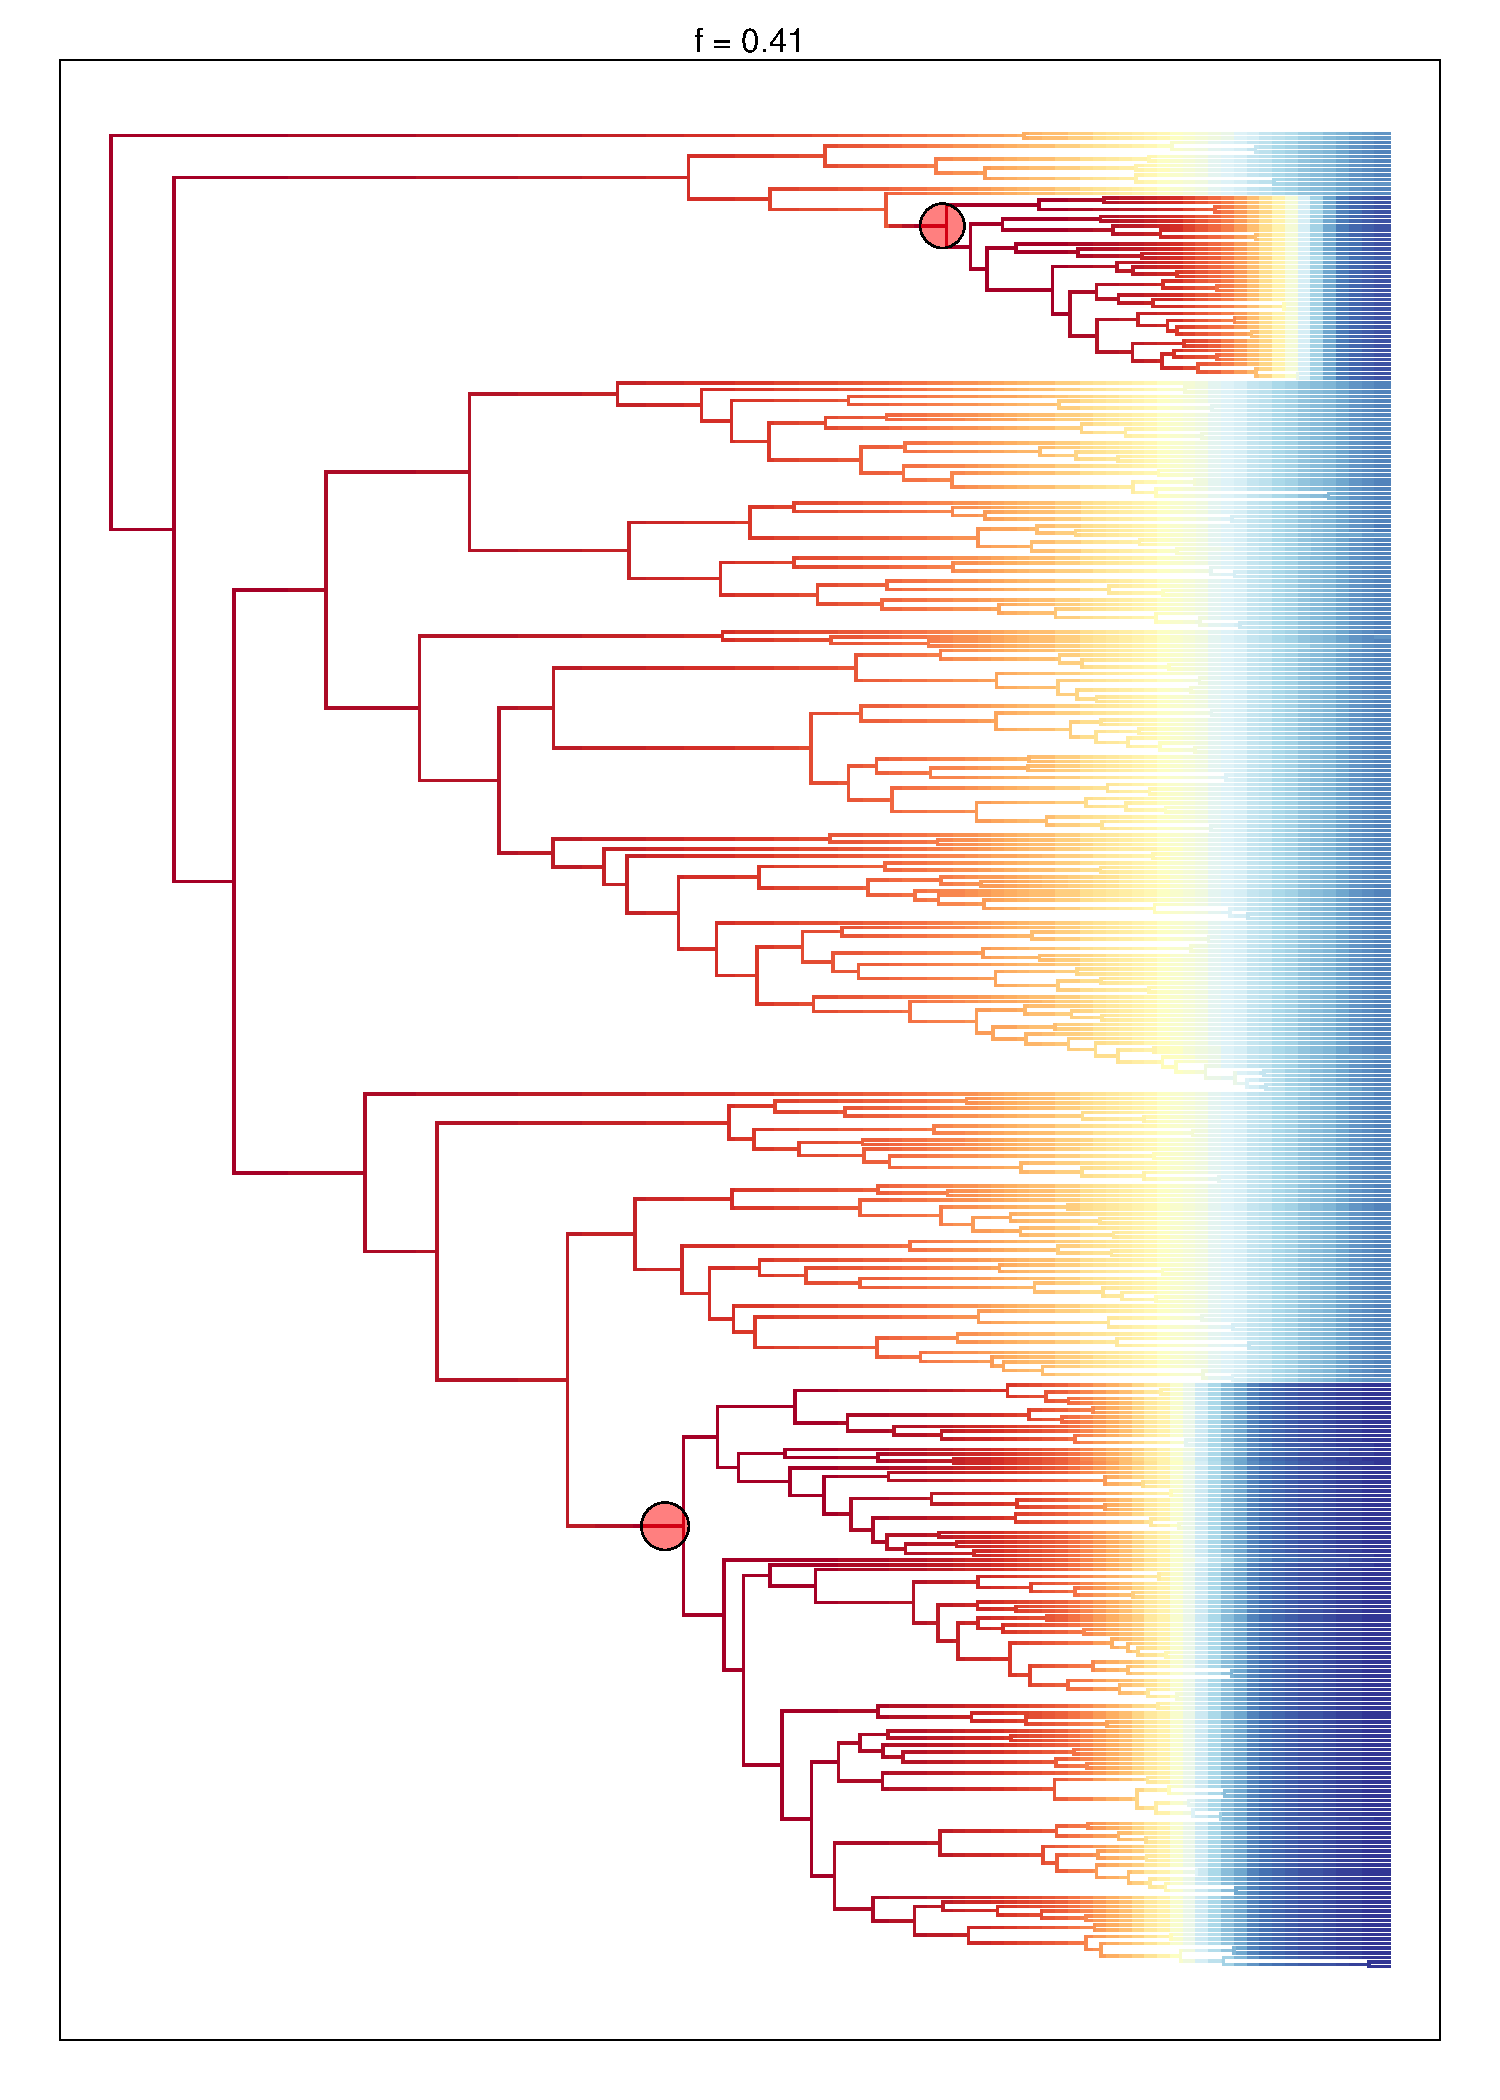
\includegraphics{response_to_reviewers_fig1.pdf}
\caption{Bamm analysis}
\end{figure}

\textbf{5. Reviewer's Comment:}

The authors should `play' with an AIC cutoff, simply to explore how it
might affect there inferences.

\textbf{5. Response:}

\begin{quote}
\color{blue}
As specified lines above and in the manuscript, we used the AIC cutoff
value 7.8 as suggested by MEDUSA (this value is regarded as optimal due
to the number of taxa in our analyses). Changing the cutoff value would
allow fewer or additional diversification shifts to be picked up by
MEDUSA. Hovewer the initial diversification shifts will remain the same
unless the AIC cutoff used is so hight that no single diversification
shifts are recovered. Thus playing with the AIC cutoff values does not
affect most of the diversification shifts discussed in our manuscript.
We rerun all our MEDUSA and MultiMEDUSA analysis with differente AIC
cutoff values to see any effect on the results. We used the AIC values 4
and 11.
\end{quote}

\begin{quote}
\color{blue}
The results in Fig.2 (also attached as PDF file) shows our MEDUSA
results from the manuscript (cutoff 7.8) along with results with AIC
cutoff values 4 and 11. We see that the first 19 diversification shitfs
are the same for cutoff values 7.8 and 4. However when using AIC cutoff
4 we recovered additional diversification shifts as the software kept
trying to fit additional models until the differente in AIC values was
less than 4. As expected MultiMEDUSA also found additinal
diversification shifts across the random sample of 1000 trees.
\end{quote}

\begin{quote}
\color{blue}
When we used AIC cutoff 11, we obtained fewer diversification shifts. We
recovered only 16, which are the same first 16 that we found in our
analysis with AIC 7.8.
\end{quote}

\begin{figure}[htbp]
\centering
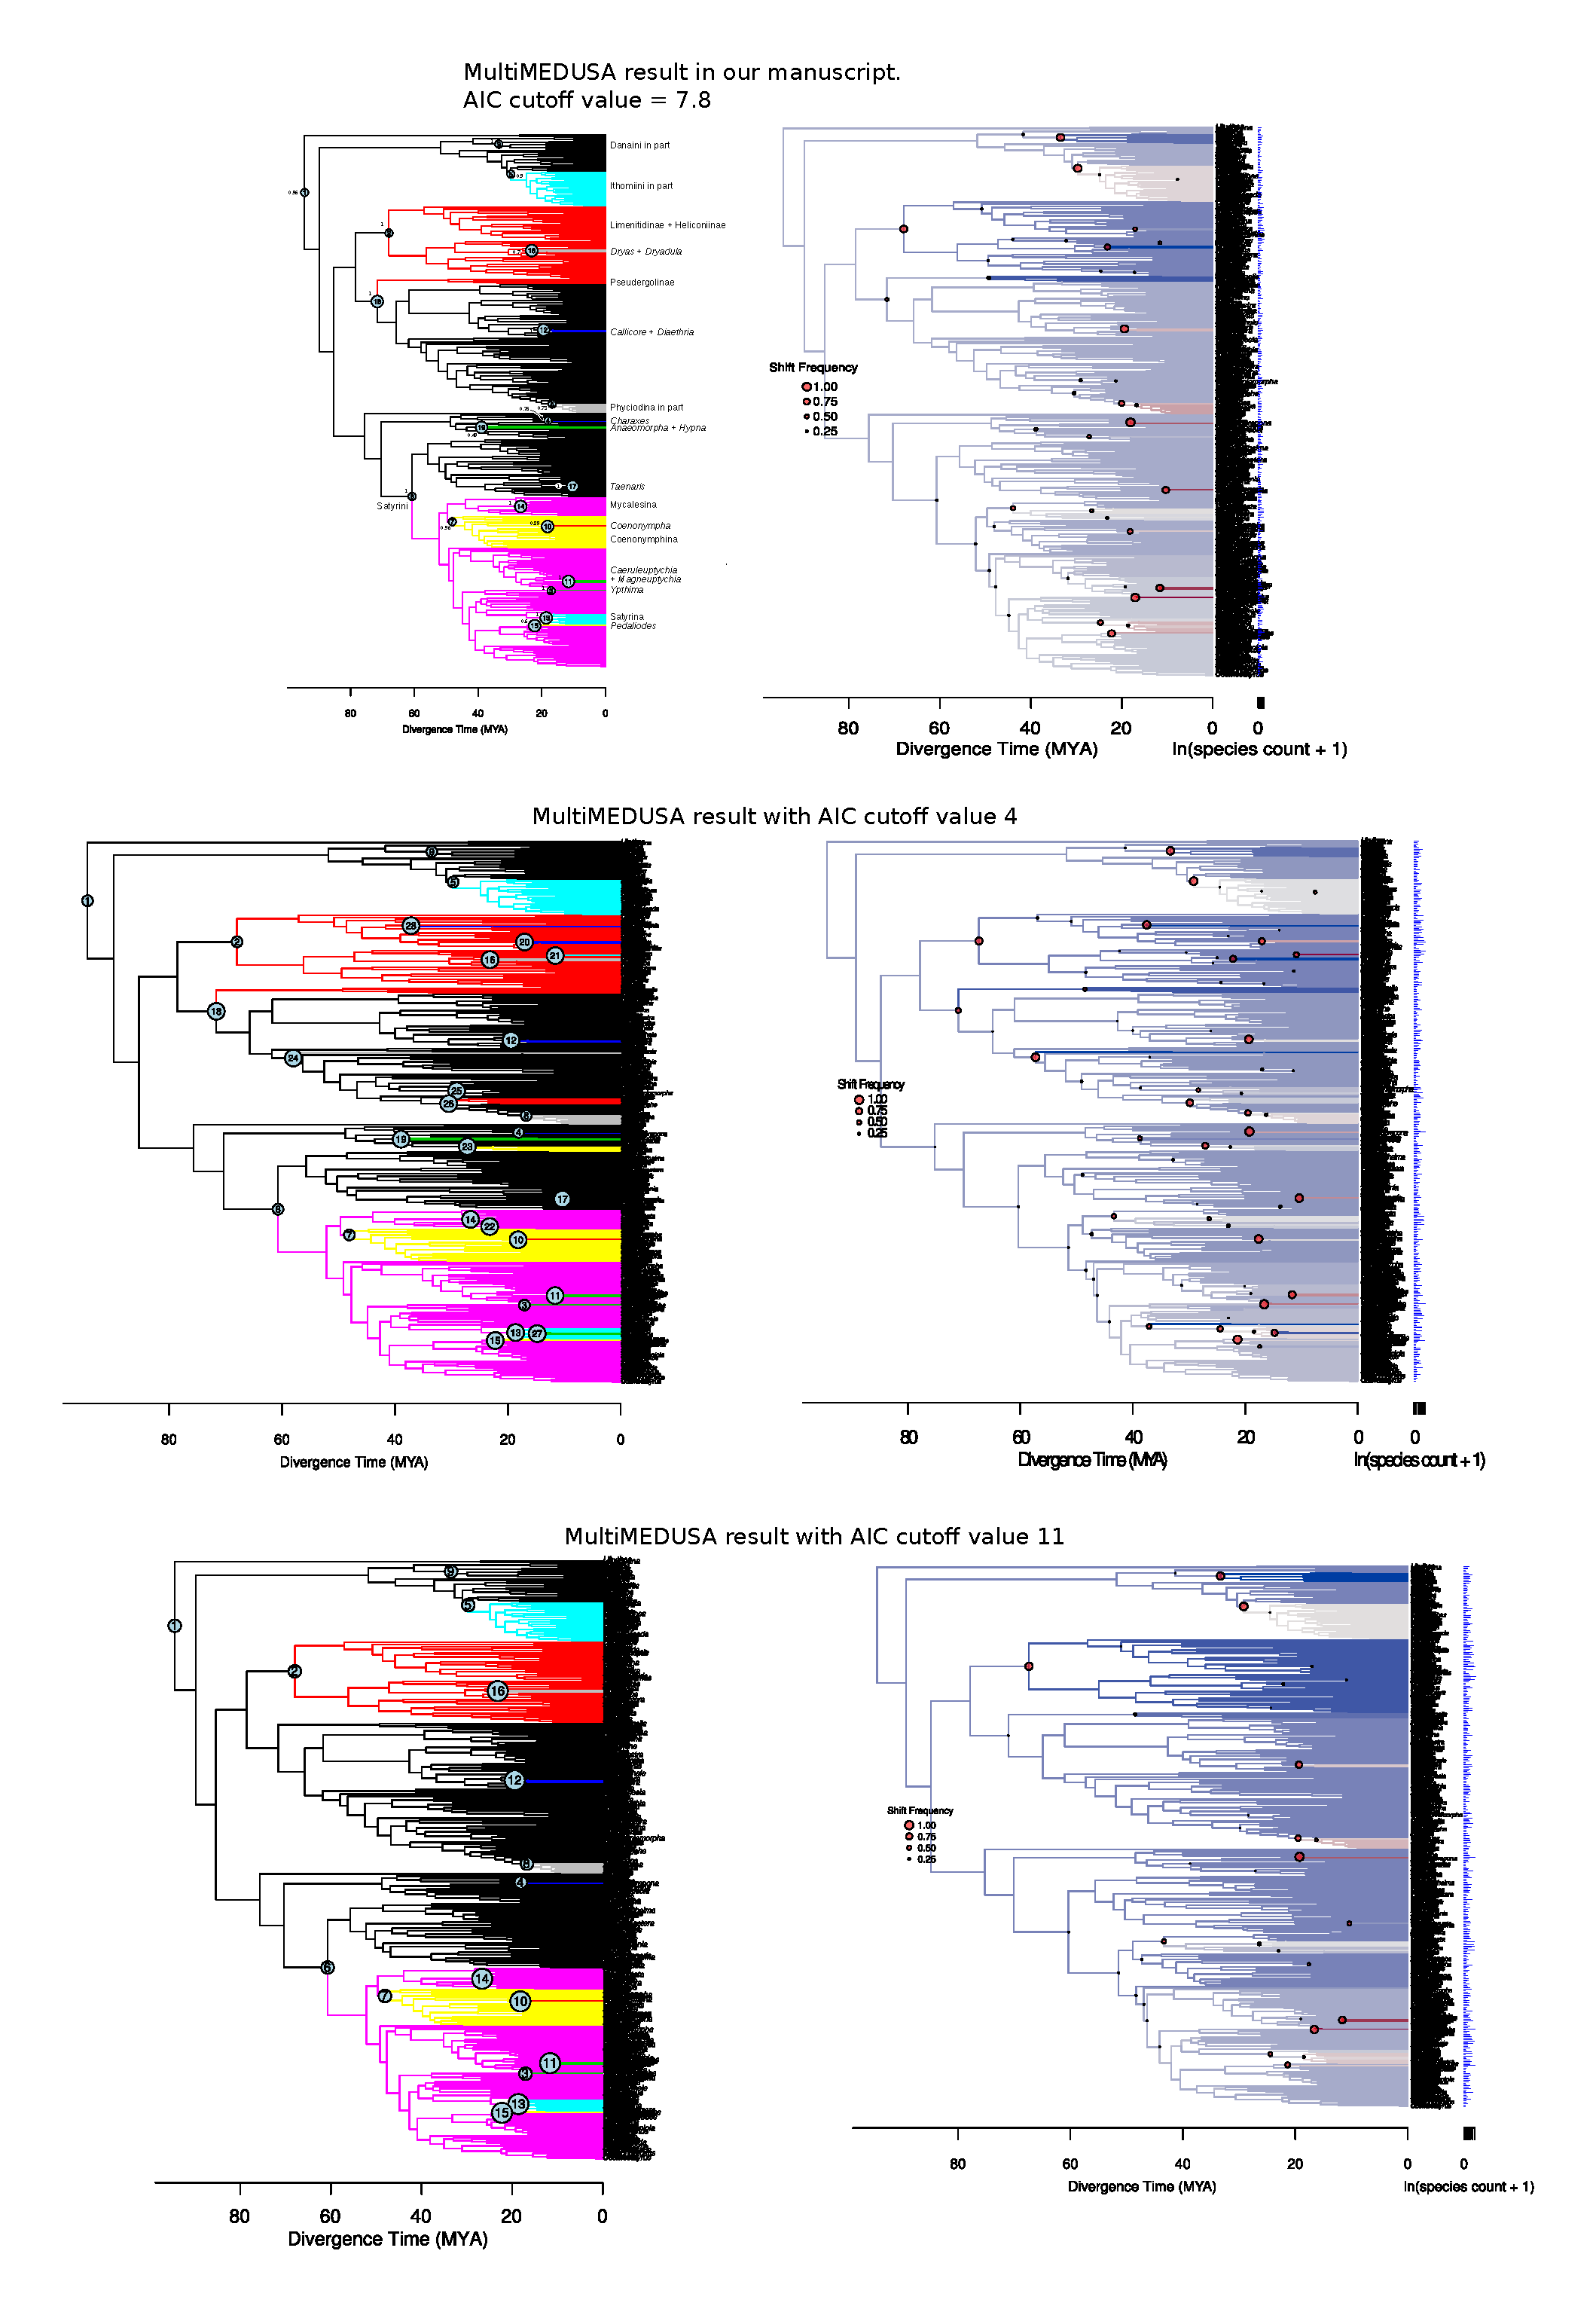
\includegraphics{multimedusa_7_8_vs_4_vs_11_AIC_cutoff.pdf}
\caption{MEDUSA analyses under three AIC values}
\end{figure}

\textbf{6. Reviewer's Comment:}

In addition, the authors should be cautious about interpreting AIC in a
frequentist manner (e.g., ``Only three out of 13 significant shifts
found on the maximum credibility tree were consistent across more than
95\% of the trees from the posterior'') -- that is, AIC is a model
selection tool, which should act as a guide for selecting the `best'
family of models. Delta AIC should really not be thought of as alpha =
0.05.

\textbf{6. Response:}

\begin{quote}
\color{blue}
We agree that AIC values should not be treated in a frequentist manner.
However, we use the term \textbf{``significant shifts''}, in the same
way as the authors of the method MEDUSA (Alfaro et al. 2009), to
pinpoint to specific nodes that show a higher net diversification rate
than ancestral or descendant nodes.
\end{quote}

\begin{quote}
\color{blue}
We also used the AIC value in the correct way. We used the cutoff 7.8
for all MEDUSA analyses. Then we counted the number of significant
shifts infered in each tree and tried to pinpoint those that were
consistently recovered across the sample of 1000 random trees (and are
also present in the MCC tree). Since no single significant shift was
found in all 1000 trees we wanted to show those are were most commonly
recovered. This is way we considered consistent diversification shifts
those that were found in most of the trees (in more than 95\% of them).
\end{quote}

\textbf{7. Reviewer's Comment:}

Why are authors referred to as references, rather than by authors.

As noted by Reference 36, the responsible trait might\ldots{}

\textbf{7. Response:}

\begin{quote}
\color{blue}
We have fixed those references as suggested by the reviewer.
\end{quote}

\section*{References}\label{references}
\addcontentsline{toc}{section}{References}

Alfaro, Michael E, Francesco Santini, Chad Brock, Hugo Alamillo, Alex
Dornburg, Daniel L Rabosky, Giorgio Carnevale, and Luke J Harmon. 2009.
``Nine Exceptional Radiations Plus High Turnover Explain Species
Diversity in Jawed Vertebrates.'' \emph{P. Natl. Acad. Sci. USA} 106
(32): 13410--14.
doi:\href{http://dx.doi.org/10.1073/pnas.0811087106}{10.1073/pnas.0811087106}.

Davis, Matthew P, Peter E Midford, and Wayne Maddison. 2013. ``Exploring
power and parameter estimation of the BiSSE method for analyzing species
diversification.'' \emph{BMC Evol. Biol.} 13 (1): 38.
doi:\href{http://dx.doi.org/10.1186/1471-2148-13-38}{10.1186/1471-2148-13-38}.

\end{document}
